\documentclass[aspectratio=169]{beamer}
%\documentclass[aspectratio=169,notes]{beamer}
%\documentclass[aspectratio=169,notes=only]{beamer}
\usepackage[english]{layout}
\usepackage[utf8]{inputenc}
\usepackage[english]{babel}
\usepackage[T1]{fontenc}
\usepackage{amsmath, soul, color, multicol, type1cm, verbatim, latexsym, dsfont, float, listings,alltt,tikz, lmodern, textcomp}
\usepackage[official]{eurosym}
\usepackage[export]{adjustbox}
\usepackage[caption = false]{subfig}
%\usepackage{beamerthemesplit}
%\usetheme{Frankfurt}
\usecolortheme{lily}
%\usefonttheme{structuresmallcapsserif}
\usefonttheme{professionalfonts}
\setbeamercovered{transparent}
\beamertemplatenavigationsymbolsempty 

\usepackage{array}

% code highlighting
\usepackage{minted}

%NeSI Colors <-------------------------------------------------------------------------------------
\usecolortheme{lily}
\usecolortheme[RGB={47, 68, 71}]{structure} 
\definecolor{nesidark}{HTML}{2F4447}
\definecolor{nesilight}{HTML}{CED9DF}
\definecolor{nesigrey}{gray}{0.7}
\definecolor{nesilightgrey}{gray}{0.98}
\definecolor{nesidarkgrey}{gray}{0.3}
\definecolor{nesiblue}{HTML}{2B9FC2}
\setbeamercolor{block title}{fg=black,bg=nesigrey}
\setbeamercolor{block body}{bg=nesilightgrey,fg=nesidarkgrey}
\setbeamercolor{block body alerted}{bg=white,fg=black}
\setbeamercolor{alerted text}{bg=white,fg=black}

\addtobeamertemplate{frametitle}{\vskip+1.2ex}{}
%NeSI Custom Code Hightlight <---------------------------------------------------------------------------------------
\lstdefinestyle{customcode}{
  belowcaptionskip=1\baselineskip,
  breaklines=true,
  xleftmargin=\parindent,
  showstringspaces=false,
  basicstyle=\ttfamily,
  keywordstyle=\bfseries\color{green!40!black},
  commentstyle=\itshape\color{purple!40!black},
  identifierstyle=\color{blue},
  stringstyle=\color{orange},
}
%NeSI Title <---------------------------------------------------------------------------------------
\setbeamerfont{title}{size=\huge}
\frenchspacing
\hyphenation{NeSI}
%NeSI Template parameters <-------------------------------------------------------------------------
\setbeamertemplate{blocks}[default]
\useinnertheme{circles}
\setbeamertemplate{title page}[default][center,rounded=false,shadow=false]
\newcommand\BackgroundPicture[1]{%
\setbeamertemplate{background}{%
\parbox[c][\paperheight]{\paperwidth}{%
\vfill \hfill \includegraphics[height=\paperheight]{#1}
\hfill \vfill
}}}

%Content Starts Here <-------------------------------------------------------------------------------
% title page
\title{Optimising a Python code with C and OpenMP}
\author[shortname]{Chris Scott \inst{1} \and Calum Chamberlain \inst{2}}
\institute[shortinst]{\inst{1} New Zealand eScience Infrastructure (NeSI) \and \inst{2} School of Geography, Environment and Earth Sciences, Victoria University of Wellington}
\date{3 August 2018}

% NeSI logo on title page
\titlegraphic{
\includegraphics[width=3cm]{NeSI/nesi_logo.png}}

\begin{document}
%\BackgroundPicture{NeSI/title.png}
\begin{frame}[plain]
%  \vspace{+3.7cm}
  \titlepage
\end{frame}

\BackgroundPicture{NeSI/blank-03.pdf}
%\BackgroundPicture{NeSI/blank_eresearch.pdf}

% This will generate the outline. If you have several topics, uncomment the multicols 
\begin{frame}
  \frametitle{Outline}
  %\begin{multicols}{2} 
  \tableofcontents
  %\end{multicols}
\end{frame}

\section{Background}

\subsection{NeSI Consultancy Service}

\begin{frame}
    \frametitle{Background}
    \framesubtitle{NeSI Scientific Programming Project}
    
    \begin{itemize}
      \item NeSI Scientific Programming Projects
        \begin{itemize}
          \item Optimise and/or parallelise code and algorithms
          \item Take advantage of accelerators (GPUs)
          \item Develop custom code
          \item Scientific data visualisation
        \end{itemize}
      \item Collaborator and merit projects
        \begin{itemize}
          \item No cost to the researcher -- already paid for
        \end{itemize}
    \end{itemize}

\end{frame}

\subsection{EQcorrscan project}


\begin{frame}
    \frametitle{Background}
    \framesubtitle{EQcorrscan}
    
    \begin{columns}
        \begin{column}{0.6\textwidth}
            \begin{itemize}
                \onslide<1->{
                    \item EQcorrscan Python package
                        \begin{itemize}
                            \item Detection and analysis of earthquakes
                            \item Developed by Calum Chamberlain
                        \end{itemize}
                }
                \onslide<2->{
                    \item Earthquake detection
                        \begin{itemize}
                            \item Small number of very long signals (seismic data) -- channels
                            \item Large number of short templates -- what an earthquake looks like
                            \item Find parts of the long signal that match any of the templates -- compute the cross correlations
                        \end{itemize}
                }
            \end{itemize}
        \end{column}
        \begin{column}{0.4\textwidth}
            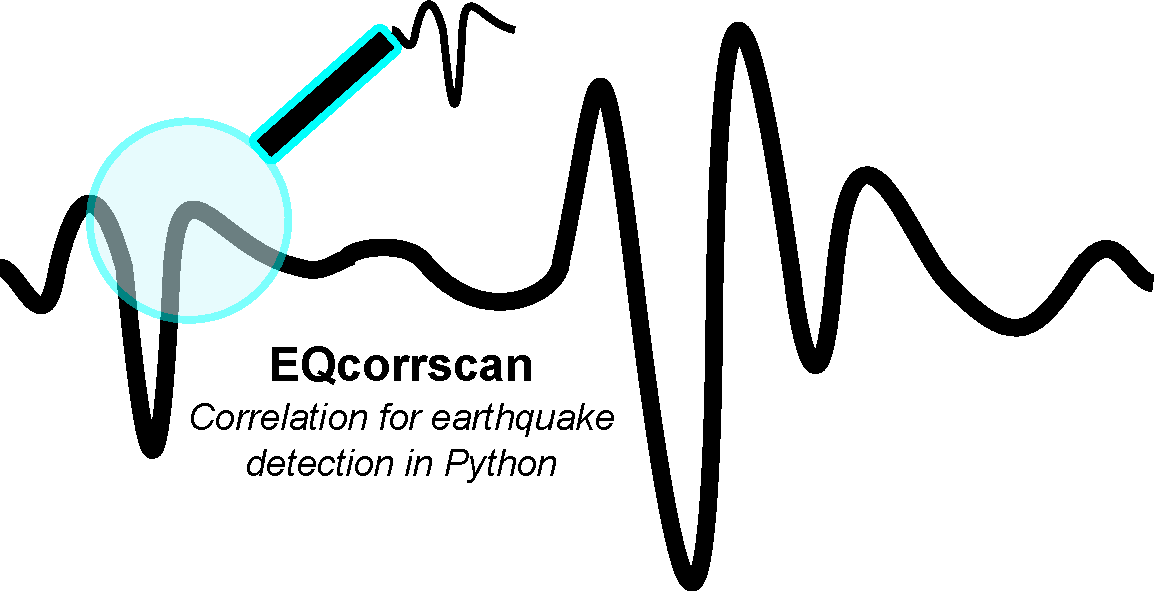
\includegraphics[width=\textwidth]{images/EQcorrscan_logo.pdf} \\
            \centering{
                \tiny{
                    EQcorrscan logo
                }
            }
        \end{column}
    \end{columns}

\end{frame}

\begin{frame}[t]
    \frametitle{EQcorrscan}
    \framesubtitle{Good practice}
    
    \centering{
        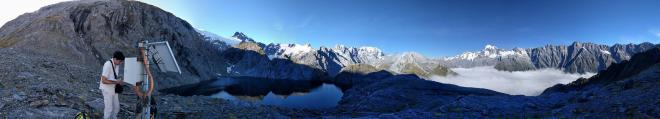
\includegraphics[width=\textwidth]{images/main-image.jpg} \\
        \tiny{
            Photo by Calum Chamberlain
        }
    }
    
    \begin{itemize}
      \item Developed on GitHub: \url{https://github.com/eqcorrscan/EQcorrscan}
        \begin{itemize}
            \item Pull requests, code review, issue tracker
        \end{itemize}
      \item Tests and continuous integration (builds on Linux, Mac, Windows)
      \item Documentation on readthedocs: \url{http://eqcorrscan.readthedocs.io}
      \item Deploys to conda-forge (anaconda) -- easy to install
      \item Easy to come in and make changes!
    \end{itemize}

\end{frame}


\section{Implementation}


\begin{frame}
    \frametitle{Aim of this project}
    
    \onslide<1->{
        \begin{itemize}
            \item Improve performance and reduce memory usage
                \begin{itemize}
                    \item Limiting the size of datasets and number of templates that can be processed
                \end{itemize}
        \end{itemize}
    }
    
    \onslide<2->{
        \begin{itemize}
            \item Initial state
                \begin{itemize}
                    \item C function to compute the cross correlations for a single channel (ctypes)
                    \item Using the FFTW library in the cross correlation calculation
                    \item Python multiprocessing loop over the channels -- calls the C function
                \end{itemize}
        \end{itemize}
    }
    
    \onslide<3->{
        \begin{itemize}
            \item Plan
                \begin{itemize}
                    \item Move outer loop into C and parallelise with OpenMP
                    \item Also parallelise the cross correlation calculation in the C function
                \end{itemize}
        \end{itemize}
    }
    
\end{frame}



\subsection{Outer loop parallelisation}

\begin{frame}
    \frametitle{Implementation}
    \framesubtitle{OpenMP for the outer loop}
    
    \begin{itemize}
      \item FFTW plans
        \begin{itemize}
            \small{}
            \item Creation is not thread safe -- must be done before the parallel loop
            \item Once allocated the plans are read-only, so can be shared by the threads
        \end{itemize}
      \item Workspace for the computation
        \begin{itemize}
            \small{}
            \item Each thread needs its own workspace (large)
            \item Memory usage grows with the number of threads
        \end{itemize}
      \item Number of channels is small ($\approx 9$)
        \begin{itemize}
            \item Cannot scale to more threads than the number of channels
        \end{itemize}
      \item Need to make sure we haven't left any Python code behind
    \end{itemize}

\end{frame}

\begin{frame}[fragile]
    \frametitle{Profiling the Python code}
    
    % do we put the graph showing time in python vs C, or the line profiler output ???
    
    \small{
        \begin{itemize}
          \item Run line profiler on the Python code (\url{https://github.com/rkern/line_profiler})
        \end{itemize}
    }
    
    \tiny{
    	\begin{minted}[frame=lines,framesep=2mm,framerule=1pt]{python}
Line   Hits   % Time  Line Contents
=====================================
 399      1      8.3  cccs = np.empty((...), np.float32).flatten(order='C')
 401      1     57.5  ret = utilslib.multi_normxcorr_fftw(...)
 408     10      0.0  for j in range(n_channels):
 409    909      0.0    for i in range(n_templates):
 410    900      0.0      if not used_chans[j][i]:
 411    593      5.5        cccs[j][i] = np.zeros(...)
 412      1      3.3  cccs[np.isnan(cccs)] = 0.0
 413      1     11.1  if np.any(np.abs(cccs) > 1.01):
 417                    raise MemoryError()
 418      1      3.3  cccs[cccs > 1.0] = 1.0
 419      1      3.3  cccs[cccs < -1.0] = -1.0
 420     10      0.0  for j, seed_id in enumerate(seed_ids):
 421    909      0.0    for i in range(len(pad_array[seed_id])):
 422    900      7.6      cccs[j][i] = np.append(...)
 426      1      0.0  return cccs, used_chans

        \end{minted}
    }
    
    \small{
        \begin{itemize}
            \item 57.5 \% time in C -- move more Python code to C so that it runs in parallel
        \end{itemize}
    }
    
    \note[item]{Simplified output from line profiler}
    \note[item]{Run on 8 threads}
    \note[item]{Python code accounting for around 40 \%}
    \note[item]{Able to move these lines into the C code to get a further boost}

\end{frame}

\begin{frame}[t]
    \frametitle{OpenMP for the outer loop}
    \framesubtitle{Benchmarks -- test case with 100 templates}
    
    \small
    
    \begin{columns}
        \begin{column}{0.6\textwidth}
            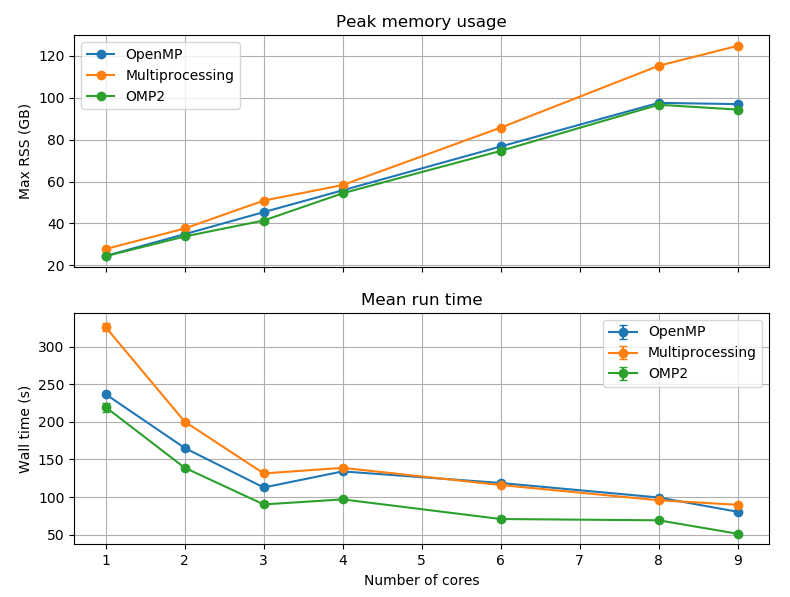
\includegraphics[width=\textwidth]{images/openmp-vs-multiprocessing-2-cropped.png}
        \end{column}
        \begin{column}{0.4\textwidth}
            \begin{itemize}
              \item OpenMP versions use slightly less memory
              \item OpenMP and Multiprocessing performance very similar (89.7 vs 80.4 seconds on 9 threads)
              \item OMP2 is fastest -- moved more Python code into C (1.8x faster than Multiprocessing and 1.6x faster than OpenMP)
            \end{itemize}
        \end{column}
    \end{columns}

\end{frame}




\subsection{Parallelising the inner function}

\begin{frame}[t]
    \frametitle{Parallelising the inner function}
    
    \begin{table}[]
        \centering
        \begin{tabular}{c|c<{\onslide<2->}|c<{\onslide}}
            Section & Initial time (s) & Improved time (s) \\ \hline
            Forward FFT & 46.8 (39.3 \%) & 6.7 (32.9 \%) \\
            Dot product & 4.0 (3.4 \%) & 1.6 (7.9 \%) \\
            Inverse FFT & 47.7 (40.1 \%) & 7.3 (35.8 \%) \\
            Normalisation & 20.0 (16.9 \%) & 4.7 (22.9 \%)
        \end{tabular}
%                \caption{Initial timings for sections of the inner function}
%                \label{tab:my_label}
    \end{table}
    
    \begin{itemize}
        \item Parallelise FFTs is easy -- use FFTW threads (and MKL FFTW interface)
        \item Dot product is a simple OpenMP loop
        \item Normalisation more complicated -- split 1 loop into 2 loops
            \begin{enumerate}
                \item First loop computes some values and store in an array (serial -- each value depends on the previous)
                \item Second loop applies the values computed in the previous step (parallel, shared memory)
            \end{enumerate}
    \end{itemize}
    
    \note[item]{Improved times running on 8 threads}
    \note[item]{Good improvement in all areas}

\end{frame}


\begin{frame}[t]
    \frametitle{Scaling}
    \framesubtitle{100 templates}

    \begin{columns}
        \begin{column}{0.4\textwidth}
            \begin{itemize}
              \item Can combine outer and inner parallelisation (nested OpenMP loops)
              \item Memory increases when adding outer threads but not inner
              \item Best performance is with 24 inner threads (lowest time and memory)
            \end{itemize}
        \end{column}
        \begin{column}{0.6\textwidth}
            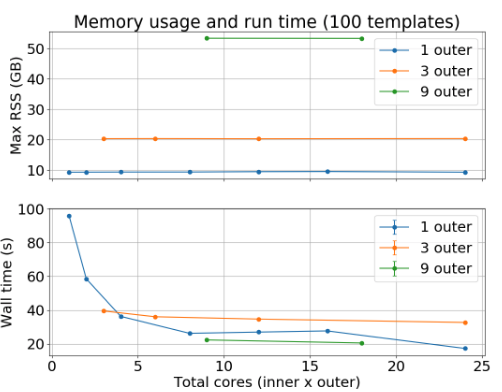
\includegraphics[width=\textwidth]{images/scaleability-100templates.png}
        \end{column}
    \end{columns}

\end{frame}

\begin{frame}
    \frametitle{Overall improvement}

    \begin{table}[]
        \centering
        \begin{tabular}{c|c|c|c}
            Version & Cores & Run time (s) & Peak memory (GB) \\ \hline
            Multiprocessing & 9 & $89.7 \pm 0.1$ & 135.6 \\
            OpenMP (double) & 9 & $44.7 \pm 0.1$ & 102.3 \\
            OpenMP (single) & 9 & $30.7 \pm 0.1$ & 53.1 \\
            OpenMP (inner) & 24 & $17.3 \pm 0.3$ & 9.3 \\
        \end{tabular}
%                \caption{Initial timings for sections of the inner function}
%                \label{tab:my_label}
    \end{table}
    
    \begin{itemize}
        \item Fastest inner threading gives 5.3x speedup over original
        \item 93 \% reduction in memory usage -- more templates can be processed at once
            \begin{itemize}
                \item Includes conversion from double to single precision
            \end{itemize}
    \end{itemize}


\end{frame}

\section{Summary}

\begin{frame}
    \frametitle{Summary}
    
    \begin{itemize}
      \item Moving Python code to C gave a good boost for this code
      \item Profile your code to make sure you pick up the important bits
      \item OpenMP -- always check thread safety of functions you call
      \item In this case, parallelising at the inner level was best -- higher core counts and lower memory usage
      \item Infrastructure around code worthwhile -- easier for collaborators to get involved
      \item Test case running over 5x faster and much lower memory usage
    \end{itemize}
    
    Check out the case study:
    \url{https://www.nesi.org.nz/case-studies/cataloguing-nz\%E2\%80\%99s-earthquake-activities}

\end{frame}

\begin{frame}
    \frametitle{Check out the other NeSI talks}
    
    \begin{itemize}
        \item Alex Pletzer, \textit{Make the most of your core hours: comparing C++/Fortran compilers on Kupe}. Thursday, 11:30am session.
        \item Mandes Schoenherr, \textit{Development tools for testing, debugging and profiling}. Friday, 11:30am session
        \item Wolfgang Hayek, \textit{In-Situ Visualisation with Paraview Catalyst}. Friday, 1:45pm session.
    \end{itemize}
    
    \vspace{1cm}
    
    \centering{
        \textbf{Talk to us to see how a consultancy project could work for you!}
    }
    
\end{frame}

\end{document}
